\documentclass[11pt]{article}
\usepackage[a4paper,margin=1in]{geometry}
\usepackage{graphicx}
\usepackage{hyperref}
\usepackage{parskip}

\title{Weekly Recap: Shuttle Path Work}
\author{}
\date{}

\begin{document}
\maketitle

\section*{Kinematic Work}
I built splines from the Excel data and extracted two path sets:
\begin{itemize}
  \item Small loop points
  \item Large loop points
\end{itemize}
These points were exported to CSV and used to drive the shuttle in kinematic mode
(\texttt{set\_pose}). Roll and pitch are fixed at zero; yaw is estimated from the path tangent
between consecutive points.

\section*{Key Observation}
Using only X, Y, Z is not sufficient for fully realistic motion. The yaw approximation
makes the rotation look simplified compared to the real shuttle.

\section*{Dynamic Attempts}
I tested several dynamic-control ideas using the CSV points as force targets, but the
behavior stayed unstable and did not converge:
\begin{itemize}
  \item oscillatory motion and unstable tracking
  \item unreliable following of the intended path
\end{itemize}
I decided to pause dynamic work and continue with kinematic mode until the system is
functionally complete. Later, I will revisit dynamics in a dedicated branch.

\section*{Implementation Notes}
\begin{itemize}
  \item Update period is clamped to 0.02 s for smooth kinematic motion.
  \item Start poses are aligned so the path passes through the shuttle pose at launch.
\end{itemize}

\newpage
\section*{Today Meeting (Concise)}
We agreed the system should not be modeled as only two fixed loops. Instead, it should be
represented as spline-based admissible paths, each tied to a specific switch configuration.
The rail topology changes with switch states, so the shuttle is allowed to move only along
the physically valid path for the current configuration.

From a control perspective, the switch states define the valid route, and the shuttle can be
represented by its progress along the active spline. When switches change, the admissible
future path changes accordingly.

If the control program selects a configuration with no valid downstream rail segment, the
simulation should not keep the shuttle on a safe trajectory. The constraint should end and the
shuttle should fall under gravity, preserving the pedagogical value of the simulation.

\section*{Next Steps}
Improve path logic to support: \\
switch-dependent routing \\
path switching based on shuttle position \\
Implement: \\
independent switch control \\
Prepare architecture for: \\
multiple shuttles \\
event-based updates \\
Later: \\
revisit dynamic simulation in a separate branch and refine it

\section*{Figures}
\begin{figure}[h]
  \centering
  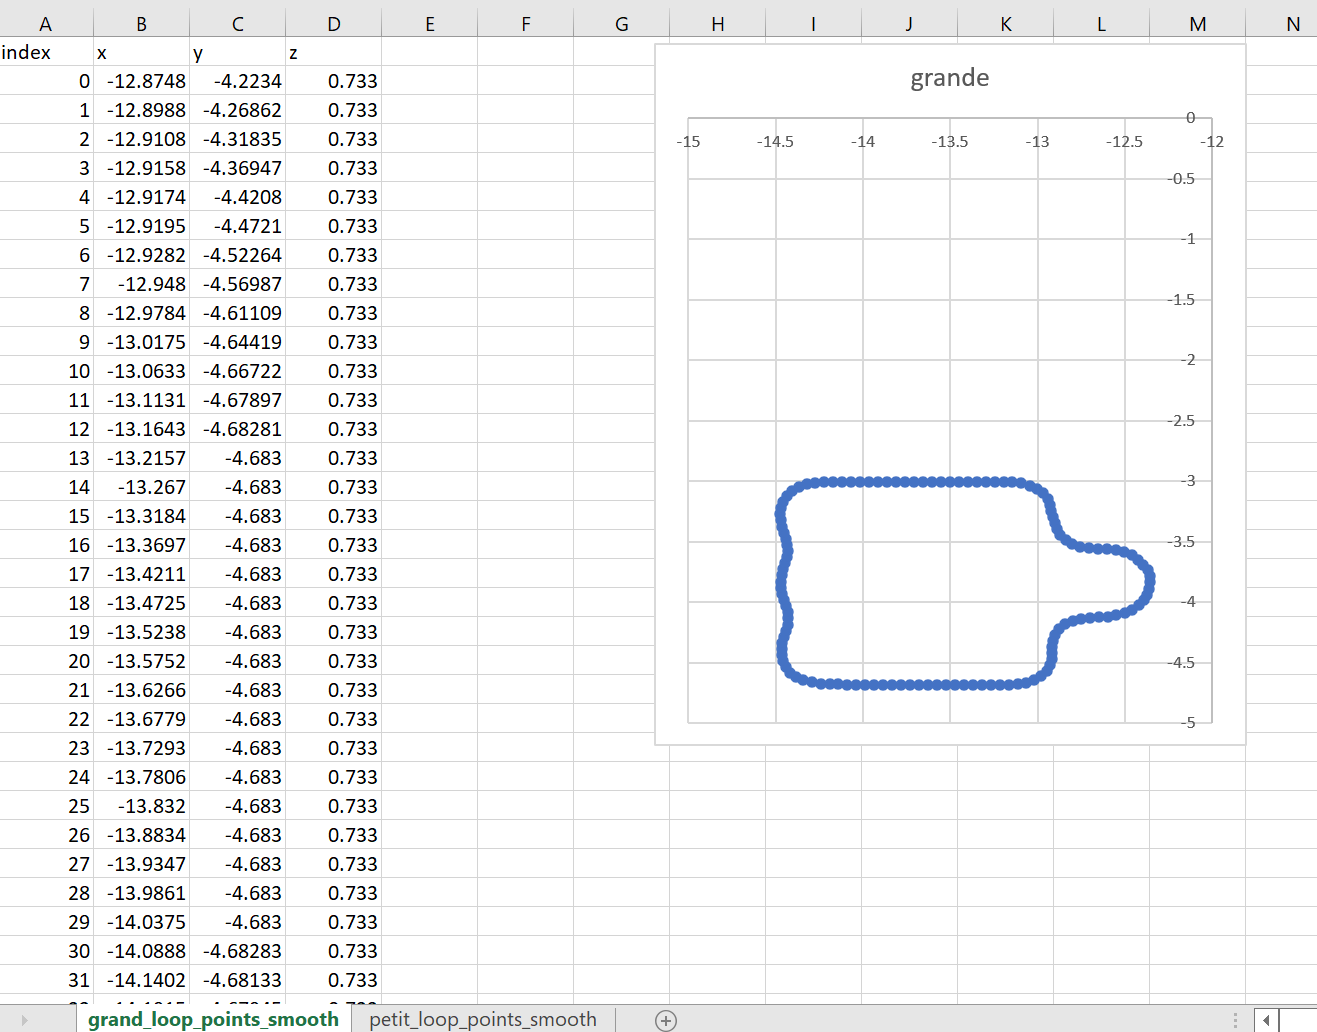
\includegraphics[width=0.8\textwidth]{grande loop.png}\\[0.45em]
  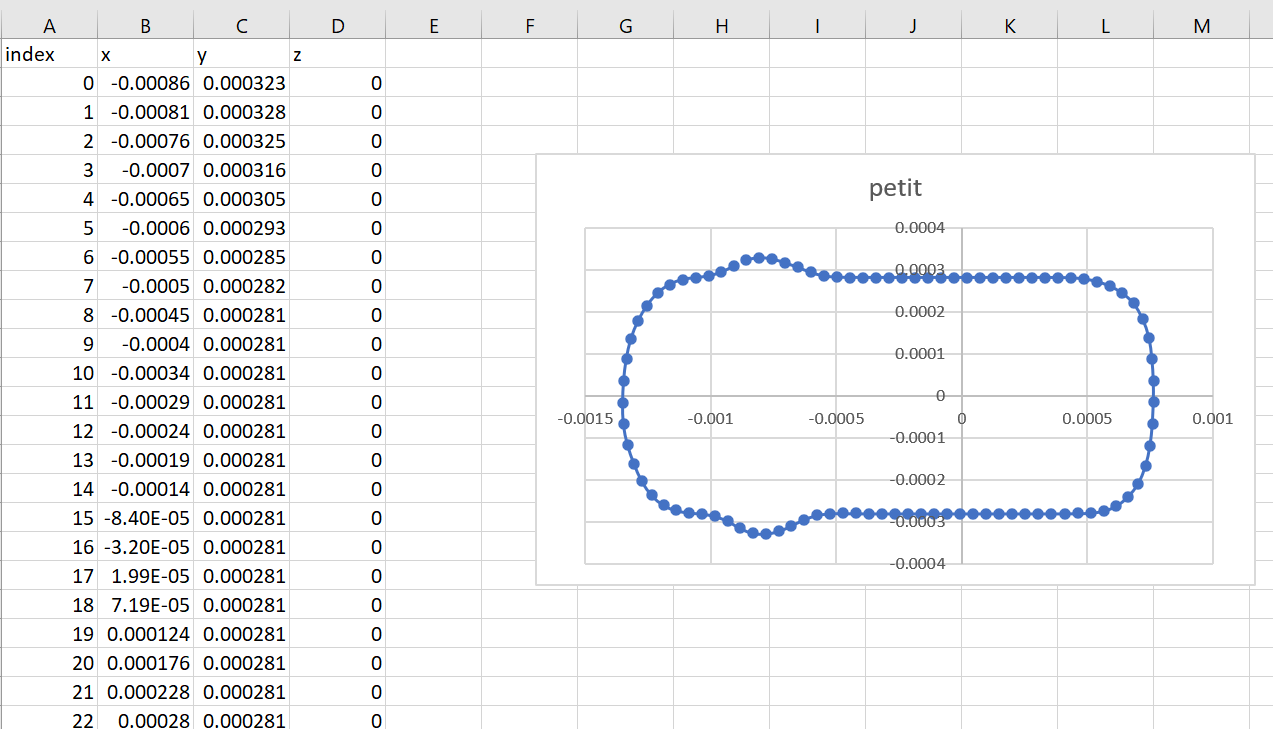
\includegraphics[width=0.8\textwidth]{petit_loop.png}\\[0.45em]
  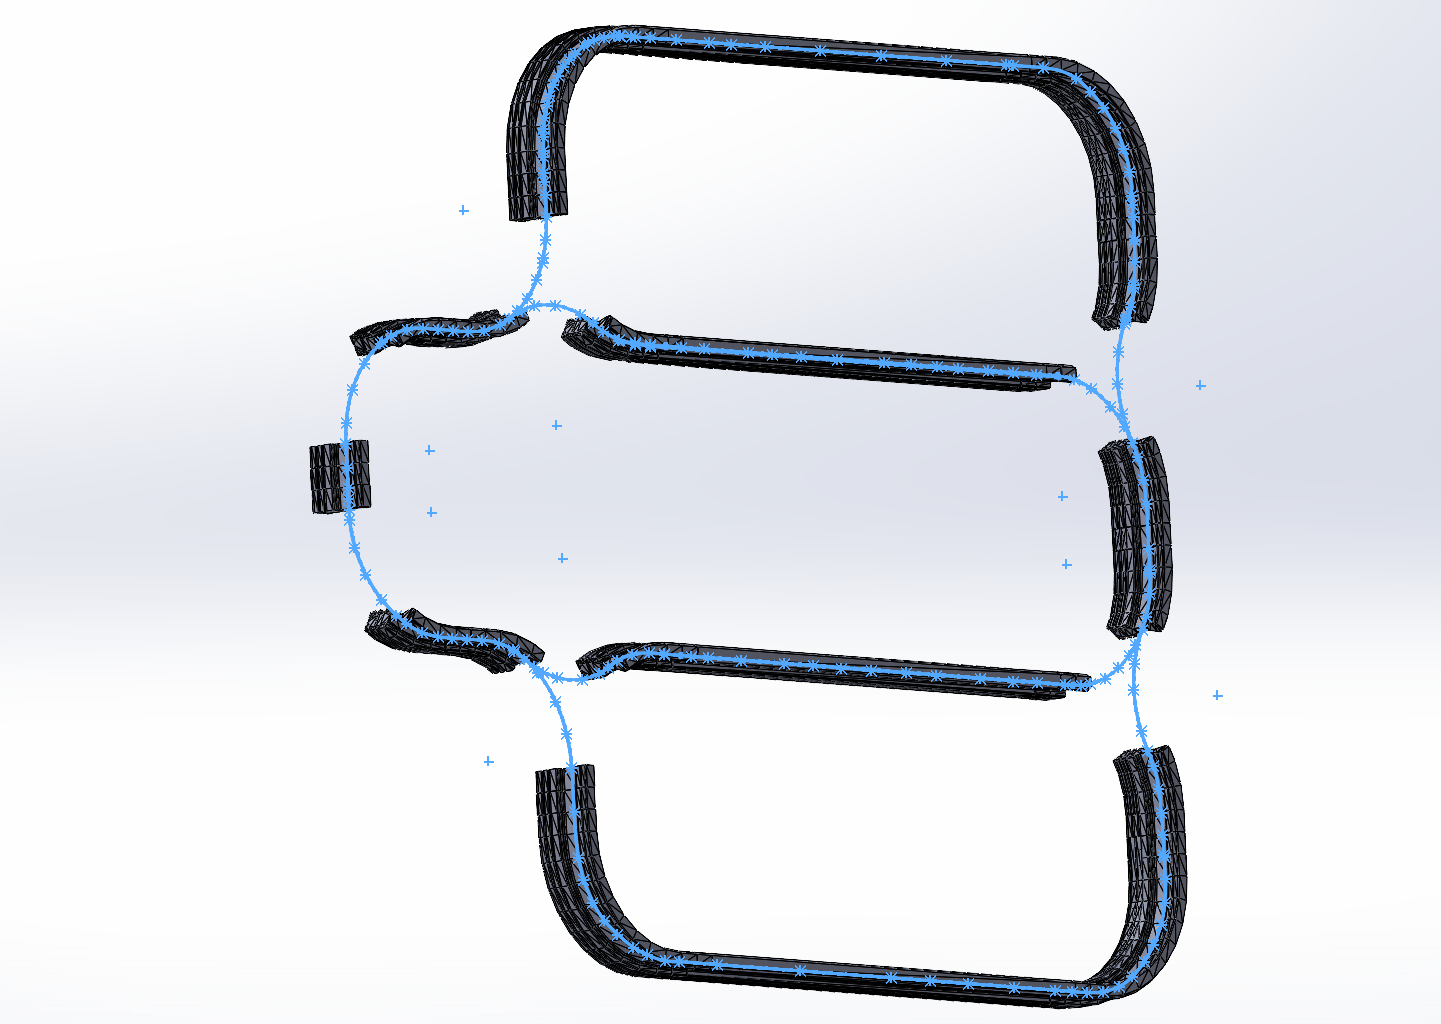
\includegraphics[width=0.8\textwidth]{solidworks points.png}
  \caption{Grand loop, petit loop, and SolidWorks reference points.}
\end{figure}

\end{document}
